\documentclass[11pt,twocolumn]{article}
\setlength{\columnsep}{0.5cm}

\usepackage[utf8]{inputenc}
\usepackage[T1]{fontenc}
\usepackage[spanish]{babel}
\usepackage{hyperref}
\usepackage{graphicx}
\usepackage{natbib}

\title{\vspace{-15mm}
	\fontsize{24pt}{10pt}\selectfont
	%\textbf{WikiPapers: a collaborative compilation of wiki research literature... in a wiki!}
	\textbf{WikiPapers: publicaciones sobre wikis recopiladas colaborativamente... ¡en un wiki!}
	}	
\author{
	\large
	\textsc{Emilio J. Rodríguez-Posada} \\
	\normalsize	Private \\
	\normalsize	\href{mailto:emijrp@gmail.com}{emijrp@gmail.com}
	\vspace{-5mm}
	}
\date{}


\begin{document}


\twocolumn[
  \begin{@twocolumnfalse}

    \maketitle

\begin{abstract}
  El interés de los investigadores por los wikis, en especial Wikipedia, ha ido en aumento en los últimos años. La primera edición de WikiSym, un simposio sobre wikis, se celebró en 2005 y desde entonces han aparecido multitud de congresos, workshops, conferencias y competiciones en este área. El estudio de los wikis es un campo emergente y prolífico. Ha habido varios intentos, aunque con escaso éxito, de recopilar toda la literatura sobre wikis. Unas veces el enfoque o la herramienta utilizada eran limitados, otras debido a las dimensiones de la tarea el proyecto era abandonado y al poco tiempo los metadatos bibliográficos se perdían. En este artículo presentamos WikiPapers, un proyecto colaborativo para recopilar toda la literatura sobre wikis. Se hace uso de MediaWiki y su extensión semántica, ambos conocidos por los investigadores de este campo. Hasta octubre de 2012 se han recopilado más de 1.400 publicaciones y sus metadatos, además de documentación sobre herramientas y datasets relacionados. Los metadatos son exportables en los formatos BibTeX, RDF, CSV y JSON. Los historiales completos del wiki están disponibles para descargar y facilitar su preservación. El proyecto está abierto a la participación de todo el mundo.
  \\
  \\
  %\textbf{Palabras clave:} literature review, collaboration, wiki, semantic wiki, Wikipedia
  \textbf{Palabras clave:} revisión de literatura, colaboración, wiki, wiki semántico, Wikipedia

\end{abstract}

  \end{@twocolumnfalse}
  ]

\section{Introducción}
El interés de los investigadores por los wikis, en especial Wikipedia, ha ido en aumento en los últimos años. La primera edición de WikiSym, un simposio sobre wikis, se celebró en 2005 y desde entonces han aparecido multitud de congresos (CLEF/PAN Lab), workshops (WikiAI, SemWiki y MathWikis), conferencias (Wikimania, WikiCon, SMWCon, Wiki Conference India, Wikipedia Academy y Wikipedia CPOV Conference) y competiciones (WikiViz). El estudio de los wikis es un campo emergente y prolífico. Ha habido varios intentos, aunque con escaso éxito, de recopilar toda la literatura sobre wikis ~\citep{ayers2011}. Unas veces el enfoque o la herramienta utilizada eran limitados, otras debido a las dimensiones de la tarea el proyecto era abandonado y al poco tiempo los metadatos bibliográficos se perdían. En este artículo presentamos WikiPapers, un proyecto colaborativo para recopilar toda la literatura sobre wikis.

El resto del artículo se divide de la siguiente manera. En la sección 2 hacemos un repaso a los distintos enfoques utilizados hasta ahora para recopilar toda la literatura sobre wikis, incidiendo en sus ventajas e inconvenientes. En la sección 3 presentamos WikiPapers, cómo funciona y qué pasos se están dando. Finalmente, en la sección 4, terminamos con unas conclusiones y trabajo futuro.

\section{Trabajos relacionados}
Ha habido distintos intentos de recopilar toda la literatura sobre wikis. Se han hecho recopilaciones en páginas personajes y blogs, a través de revisiones de literatura, haciendo uso de gestores de bibliografía, en páginas de Wikipedia y también en servicios como Zotero o CiteULike. A continuación los describimos y evaluamos sus ventajas e inconvenientes y cómo WikiPapers resuelve las carencias de estos enfoques.

\subsection{Páginas personales y blogs}
Algunos autores han hecho recopilaciones de literatura en webs personales\footnote{\href{http://www.public.iastate.edu/~CYBERSTACKS/WikiBib.htm}{http://www.public.iastate.edu/~CYBERSTACKS/WikiBib.htm}} y blogs. Un ejemplo bastante completo de este último tipo es SWEETpedia,\footnote{\href{http://www.mkbergman.com/sweetpedia/}{http://www.mkbergman.com/sweetpedia/}} que contiene publicaciones sobre wikis y semántica. Uno de los inconvenientes de este sistema es que el esfuerzo suele recaer sobre una única persona y los metadatos no son fácilmente exportables. En WikiPapers el trabajo se hace colaborativamente y todos los metadatos son fácilmente exportables en diversos formatos.

\subsection{Gestores bibliográficos en servidores propios}
Se han empleado gestores bibliográficos específicos como WIKINDX\footnote{\href{http://sourceforge.net/projects/wikindx/}{http://sourceforge.net/projects/wikindx/}} creando portales como Wikibibliographie ENCYCLEN\footnote{\href{http://wikindx.inrp.fr/biblio_encyclen/}{http://wikindx.inrp.fr/biblio\_encyclen/}} pero, como contrapartida, decidieron restringir la edición a un círculo de usuarios aprobados. En WikiPapers, sin embargo, pueden participar tanto usuarios registrados como sin registrar.

%\href{http://toolserver.org/~voj/bibliography/}{http://toolserver.org/~voj/bibliography/}
%\href{http://wikiindex.org/Wiki_Research_Bibliography}{http://wikiindex.org/Wiki\_Research\_Bibliography}

\subsection{Revisiones de literatura}
Se han realizado varias revisiones de literatura hasta ahora, con diferente grado de exhaustividad. La primera de ellas ~\citep{voss2005} se hizo en un momento en el que las publicaciones eran escasas, pero ya se podía ver una tendencia de publicación creciente y muchas preguntas por responder. Un año más tarde ~\citep{ayers2006} vuelve a hacer un repaso a la literatura existente y enumera aquellas áreas que han recibido interés: historiales, páginas de discusión, contenido de los artículos, políticas del sitio, citas a artículos, encuestas a usuarios y listas de correo.

No sería hasta 3 años después cuando ~\citep{okoli2009b} presentan una propuesta de protocolo para hacer un mapeo sistemático de la literatura sobre Wikipedia, indicando la existencia de más de 1.000 publicaciones y ese mismo año ~\citep{okoli2009} analiza el estado del arte. Dos años más tarde, ~\citep{nielsen2011} hace la mayor revisión de literatura en un documento de más de 50 páginas, en progreso e inacabado, que incluye 300 referencias a publicaciones y reincide en la existencia de 1.000 publicaciones sobre el tema.

~\citep{martin2011}

~\citep{okoli2012}

~\citep{jullien2012}

Uno de los inconvenientes de estas revisiones de literatura es que quedan rápidamente desactualizadas debido al ritmo con el que aparecen nuevas publicaciones. WikiPapers es actualizado continuamente por su comunidad de voluntarios.

\subsection{Recopilaciones en Wikipedia}
También existen listados de publicaciones y recursos en algunas Wikipedias, como en la versión alemana\footnote{\href{http://de.wikipedia.org/wiki/Wikipedia:Wikipedistik/Bibliographie}{http://de.wikipedia.org/wiki/Wikipedia:Wikipedistik\\ /Bibliographie}} y la inglesa\footnote{\href{http://en.wikipedia.org/wiki/Wikipedia:Academic_studies_of_Wikipedia}{http://en.wikipedia.org/wiki/Wikipedia:Academic\\ \_studies\_of\_Wikipedia}}. El principal inconveniente de este enfoque es que no es posible jugar con los datos dentro del mismo wiki, al estar todo escrito como texto plano, sin enriquecimiento semántico. En WikiPapers todos los metadatos son propiedades semánticas, tanto en las llamadas infoboxes (tablas) como en el cuerpo del artículo.

\subsection{Servicios web y redes sociales}
Finalmente, existen servicios web y redes sociales con recopilaciones de literatura sobre wikis. Es el caso de grupos de Zotero,\footnote{\href{https://www.zotero.org/groups/wikipedia_research}{https://www.zotero.org/groups/wikipedia\_research}} tags de BibSonomy\footnote{\href{http://www.bibsonomy.org/tag/wikipedia}{http://www.bibsonomy.org/tag/wikipedia} y \href{http://www.bibsonomy.org/tag/wiki}{http://www.bibsonomy.org/tag/wiki}} y grupos y tags de CiteULike.\footnote{\href{http://www.citeulike.org/tag/wikipedia}{http://www.citeulike.org/tag/wikipedia}, \href{http://www.citeulike.org/tag/wiki}{http://www.citeulike.org/tag/wiki} y \href{http://www.citeulike.org/group/382}{http://www.citeulike.org/group/382}} Este enfoque sí hace uso de una comunidad de usuarios para procesar las publicaciones, pero de nuevo requieren registrarse, y la capacidad para aprovechar los metadatos generando tablas o gráficos es nula.

\section{WikiPapers}
WikiPapers\footnote{\href{http://wikipapers.referata.com}{http://wikipapers.referata.com}} fue lanzado en abril de 2011. Haciendo uso de MediaWiki y su extensión semántica, recopila de manera colaborativa información acerca de toda la literatura científica sobre wikis, así como de herramientas y datasets relacionados. No hace falta estar registrado para participar, pero es recomendable.

WikiPapers agrupa todas las ventajas de los sistemas mencionados anteriormente y soluciona sus inconvenientes. Permite hacer listados de publicaciones similares a SWEETpedia: existe uno de revisiones de literatura por poner solo un ejemplo.\footnote{\href{http://wikipapers.referata.com/wiki/List_of_literature_reviews}{http://wikipapers.referata.com/wiki/List\_of\\ \_literature\_reviews}} Funciona como un gestor bibliográfico, al almacenar los metadatos de las publicaciones y permitir hacer búsquedas, filtrarlos o exportarlos, individualmente o en conjunto. También facilita que grupos de usuarios se comuniquen a través de las páginas de discusión y compartan información sobre publicaciones de su interés, funcionando como una red social. Por otro lado, el espacio de discusión debajo de cada página posibilita a los lectores hacer valoraciones de los artículos.

Desde un punto de vista más estadístico, es posible generar gráficas a partir de los metadatos disponibles en WikiPapers, aprovechando así la capacidad que ofrece la semántica. Gráficos de barras, circulares o líneas temporales están presentes y facilitan la visualización y comprensión de la información. También existe la posibilidad de incrustar diapositivas (SlideShare) y vídeos (YouTube, Vimeo).

Finalmente, el wiki y sus historiales están disponibles tanto para su descarga como dump XML y accesible a través de la API de MediaWiki. Esto impide que todo el trabajo se pierda, como ha sucedido en otros proyectos.

\begin{figure}[htb]
\centering
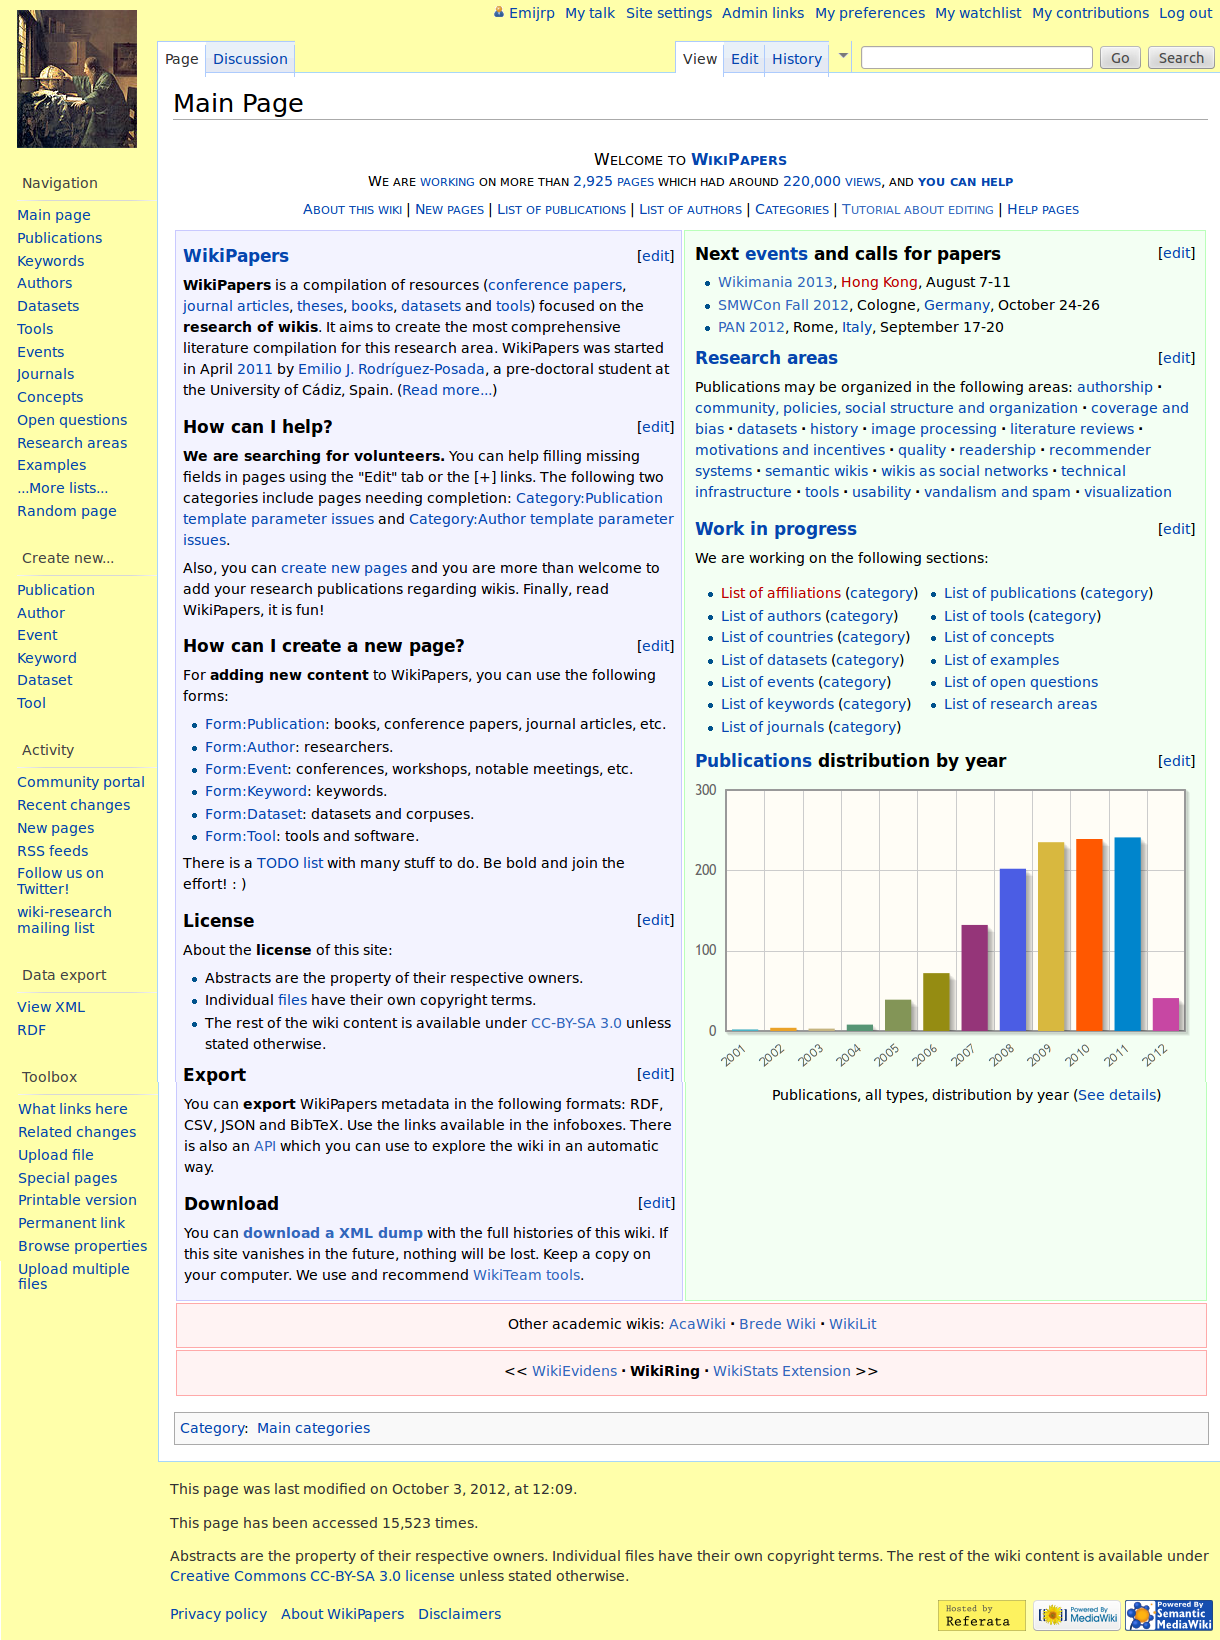
\includegraphics[width=0.49\textwidth]{wpfull.png}
\caption{Portada de WikiPapers}
\label{fig:wpfull}
\end{figure}

\subsection{Publicaciones}
En WikiPapers cada publicación dispone de una página en la que se detallan todos sus metadatos (título, autores, palabras clave, año, revista o congreso, DOI, idioma, licencia, enlaces al fichero y motores de búsqueda), el abstract, las referencias que incluye y las citas que recibe, y un espacio de discusión. Los metadatos sirven para hacer búsquedas y filtrar los contenidos. A octubre de 2012 ya cuenta con más de 1.400 publicaciones,\footnote{\href{http://wikipapers.referata.com/wiki/List_of_publications}{http://wikipapers.referata.com/wiki/List\_of\_publications}} incluyendo artículos de revistas y congresos, tesis y libros. Todos los metadatos se pueden exportar en los formatos BibTeX, RDF, CSV y JSON.

\subsection{Palabras clave}
Existe un listado de todas las palabras clave\footnote{\href{http://wikipapers.referata.com/wiki/List_of_keywords}{http://wikipapers.referata.com/wiki/List\_of\_keywords}} presentes en los artículos y cada una de ellas cuenta con varios términos relacionados, lo que permite navegar entre ellas. Las más frecuentes son: Wikipedia, wiki, semantic wiki, web 2.0, collaboration, evaluation, collaborative learning, knowledge management, MediaWiki, motivation, data mining y conflict. 

\subsection{Autores}
Para cada autor existe una ficha que incluye su nombre, afiliación, país, índice de coautores, página web, estadísticas sobre número de publicaciones y citas, y por supuesto un listado de publicaciones, datasets y herramientas de su creación. Ya están listados unos 1.000 autores.\footnote{\href{http://wikipapers.referata.com/wiki/List_of_authors}{http://wikipapers.referata.com/wiki/List\_of\_authors}}

\subsection{Datasets}
Un listado de datasets\footnote{\href{http://wikipapers.referata.com/wiki/List_of_datasets}{http://wikipapers.referata.com/wiki/List\_of\_datasets}} permite observar la gran cantidad de datos sobre comunidades wiki disponibles para analizar. Existen datasets sobre vandalismo, texto wiki enriquecido con semántica, datos extraidos de infoboxes, logs anonimizados de visitas, mensajes de listas de correo y por supuesto los típicos dumps de Wikipedia.

A este respecto, el proyecto WikiTeam\footnote{\href{http://code.google.com/p/wikiteam/}{http://code.google.com/p/wikiteam/}} está compilando una gran cantidad de datos sobre comunidades wiki, que se cifra ya en 4.500 dumps.

\subsection{Herramientas}
Se está construyendo un listado de herramientas\footnote{\href{http://wikipapers.referata.com/wiki/List_of_tools}{http://wikipapers.referata.com/wiki/List\_of\_tools}} que se han desarrollado y usado a la hora de investigar sobre wikis. Entre ellas se incluyen:

\begin{itemize}
\item \textbf{Anti-vandalismo:} AVBOT, Clue Bot, CryptoDerk's Vandal Fighter, Huggle, Igloo, STiki, Salebot, Twinkle, Vandal Fighter, VandalProof, VandalSniper.
\item \textbf{Estadística y visualización:} HistoryFlow, StatMediaWiki, Wiki Explorator, Wiki Trip, WikiEvidens, WikiTrust.
\item \textbf{Framework:} Java Wikipedia Library, Perlwikipedia, pywikipedia.
\item \textbf{Lenguaje:} Manypedia, Wikokit, Zawilinski.
\item \textbf{Preservación:} WikiTeam tools.
\item \textbf{Procesamiento de datos:} DiffDB, Ikiwiki, Infobox2rdf, Wiki Edit History Analyzer, Wikihadoop, Wikipedia Miner.
\end{itemize}

La lista no es exhaustiva y está en continuo crecimiento.

\subsection{Y más...}
También se está recopilando información sobre revistas, congresos, eventos, conceptos, ejemplos de análisis, preguntas abiertas, encuestas, motores wiki, wikifarms y más. WikiPapers, además de todo lo comentado anteriormente, es un lugar donde investigadores hacen comunidad y establecen conexiones para futuras investigaciones.

\section{Conclusiones y trabajo futuro}
El estudio de los wikis es un campo emergente y prolífico. Hasta ahora se habían tomado distintos enfoques a la hora de recopilar toda la literatura sobre este tema. Se habían utilizado webs personales y blogs (SWEETpedia), gestores bibliográficos (WIKINDX), servicios web y redes sociales (Zotero, BibSonomy, CiteULike), pero cada uno tenía sus ventajas e inconvenientes.

En este artículo hemos presentado WikiPapers, un proyecto colaborativo para recopilar toda la literatura sobre wikis. Se hace uso de MediaWiki y su extensión semántica, ambos conocidos por los investigadores de este campo. Hasta octubre de 2012 se han recopilado más de 1.400 publicaciones y sus metadatos, además de documentación sobre herramientas y datasets relacionados. Los metadatos son exportables en los formatos BibTeX, RDF, CSV y JSON. Los historiales completos del wiki están disponibles para descarga y facilitar su preservación.

\bibliographystyle{wink}
\bibliography{wikipapers-2012}

\section*{Agradecimientos}


\section*{Licencia}
Esta obra tiene licencia \href{http://creativecommons.org/licenses/by-sa/3.0/}{Creative Commons Reconocimiento-CompartirIgual 3.0 Unported}.

\end{document}
